\documentclass[12pt,a4paper,titlepage,final]{report}
% \documentclass{report}

\usepackage[czech]{babel}
\usepackage[utf8]{inputenc}
\usepackage[T1, IL2]{fontenc}
\usepackage[scale=0.7,vmarginratio={1:2},heightrounded]{geometry}

\title{FYO - Fyzikální optika\\Wienerův pokus foo}
\author{Marek Salát, xsalat00}
\date{\today}

\usepackage[bookmarksopen,colorlinks,plainpages=false,urlcolor=blue]{hyperref}
\usepackage{url}

\usepackage{natbib}
\usepackage{graphicx}
\usepackage{epstopdf}
\usepackage{wrapfig}

\usepackage{lipsum}
\usepackage{xcolor}
\usepackage{caption}
\usepackage{subcaption}
\usepackage{listings}
\usepackage{verbatim}

\graphicspath{ {./figures/} }

\renewcommand{\thesection}{\arabic{section}}%
\newcommand\todo[1]{\textcolor{red}{#1}}

\begin{document}
\lstset{language=Matlab}

\maketitle

\pagestyle{plain}
\pagenumbering{roman}
\setcounter{page}{1}
\tableofcontents

\newpage
\begin{abstract}
\todo{Justify your choices, i.e., justify reasons to end up to classifier and feature extraction technique you were using.}
\end{abstract}

\newpage
\pagestyle{plain}
\pagenumbering{arabic}
\setcounter{page}{1}

\section{Úvod}
\todo{nejak dat dohromadz spodni odstavec aby to bylo jasné, ale pozor, preklad je uz v textu}
By 1890, then, scientists were interested in studying standing waves of light: it seems that a number of them remained unconvinced that light truly was just another manifestation of electromagnetic waves! One big obstacle stood in the path of such studies: the smallness of the wavelength of light. Hertz’s radio waves had a wavelength of meters, but visible light has a wavelength on the order of 500 nanometers, or 500 billionths of a meter! Such distances cannot be directly observed with the naked eye, so experimental ingenuity was required – and Otto Wiener provided it.

As we will see, there is some irony associated with Weiner’s work. The majority of the paper is devoted to experiments relating to the so-called “mechanical theory of light”, the idea (invalidated by Einstein’s relativity) that light waves are in fact an oscillation of some as yet undiscovered material medium, dubbed the “aether”. The most important part of Weiner’s work, the interpretation of his results in the context of electromagnetic theory, seems almost an afterthought in the paper!

Wiener’s name is linked with the experimental demonstration of standing light waves. In 1888 Heinrich Hertz, working in the physics institute of the Technische Hochschule of Karlsruhe, proved the existence of electromagnetic waves. Those he detected had lengths of about eight meters. A year later Wiener performed a similar experiment with light waves–electromagnetic waves–approximately ten million times shorter than those used by Hertz. In the simplest case these waves arise in front of a plane metal mirror from the interference of incident monochromatic waves with the reflected ones
 
\section{Otto Wiener}
% http://www.encyclopedia.com/doc/1G2-2830904649.html
% http://en.wikipedia.org/wiki/Otto_Wiener_%28physicist%29

Otto Wiener se narodil roku 1862 učiteli deskriptivní geometrie na Karlsruheské střední škole Christianu Wienerovi 
a matce Paulíně Hausrathové (sestra protestantského kněze). Wienerova matka zemřela na tyfus. Chlapec osiřel ve věku tří let. \cite{encyclopedia_otto}

\begin{figure}[!htb]
	\centering
	\begin{subfigure}[b]{0.4\textwidth}
 		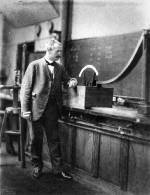
\includegraphics[width=\textwidth]{Otto_Wiener}
	\end{subfigure}
	~ %add desired spacing between images, e. g. ~, \quad, \qquad, \hfill etc.
      %(or a blank line to force the subfigure onto a new line)
	\begin{subfigure}[b]{0.4\textwidth}
 		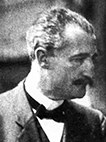
\includegraphics[width=\textwidth]{Otto_Wiener_mini}
	\end{subfigure}
	
	\caption{Otto Wiener, experimentální fyzik v Lipsku od roku 1899.}\label{fig:otto}
\end{figure}       

Wiener studoval nejdříve v Karlsruhe, poté se přesunul do Berlína, nakonec získal doktorát na Štrasburské univerzite v roce 1887
pod vedením Augusta Kundta za práci, která se zabívala změnou fáze (elekrické šložky) světla při odrazu. V roce 1890 se stal kvalifikovaným lektorem "Stehende Lichtwellen" (stojaté vlny). Wiener je znám předevsím pro přínos v oblasti stojatých vln a také proto, že byl schopen změřit 
vlnovou délku světla (mimo jiné také šířku půhledného filmu). V roce 1895 byl povýšen a ve stejném roce (ve věku 32 let) se oženíl s Linou Fennerovou. 
Roku 1895 Wiener přijal nabídku plného profesoriátu na Guessenské univerzitě. Jeho cílem zde bylo vybudovat nový institut fyziky. 
Zkušenosti z toho projektu využil v podobném projektu Lipské univerzity v roce 1899. \cite{encyclopedia_otto}

Jak bylo napsáno výše Wienerovo jméno je povětšinou spojováno s experimetny, které demonstrují stojaté vlny. V roce 1888 Heinrich Hertz
prokázal v Karlsruhelském institutu existenci elektromagnetických vln. Vlny, které detekoval, měly délku okolo osmi metrů. Rok později Wiener
provedl podobný experiment s elektromagnetickými vlnami světla, které jsou přibližně milionkrát menší než vlny, které detekoval Hertz. \cite{encyclopedia_otto}

Poté co obdržel doktorát, bylo jeho cílem změřit absobrci světla na tenké pruhledné kovové vrstvě. K provedení bylo zapotřebí znát šířku
vrstvy a změnu fáze světla při reflekci (odrazu). Díky tomuto výzkumu se stal Wiener průkopníkem v této oblasti. \cite{encyclopedia_otto}

Stojaté vlny brzny nalezly upatnení v Lippmannové barevné fotografii. Wiener měl také zálibu v technických problémech, především v letu ptáků, 
a byl velmi zaujat v leteckým průmyslem. Otto Wiener zemřel roku 1927 v neměckém Lipsku ve věku šedesáti čtyř let. \cite{wiki_otto}

\section{Stojaté vlny}
V roce 1890, byla myšlenka, že je světlo tvořeno elekromagnetickými
vlnami realtivne nová. J. C. Maxwell dokázal, že se elektromagnetické vlny šíří rychlostí světla. První člověk, který
byl toto schopen demonstrovat a dokázal existenci elekromagnetických vlny byl Heinrich Hertz. V roce 1887 dokázal, že jsou tyto vlny
konzistetní s Maxwellovou teorii, dokázal měřit jejich rychlost,
intenzitu elekrickeho pole a polarizaci. Dokonce se mu i 
podařilo vytvoři stojatou vlnu za pomocí zinkové destičky. \cite{skullsinthestars}

Stojatá vlny vniká je monochromatická vlny odražena z povrchu, odražená vlna pak interferuje s vlnou pricházející a vznikne tak 
vlny která osciluje nahoru a dolů bez zdálivého směru pohybu. 
Tento je je znázorněn na následují serii obrázku.

\begin{figure}[!h]
        \centering
        \begin{subfigure}[b]{0.23\textwidth}
                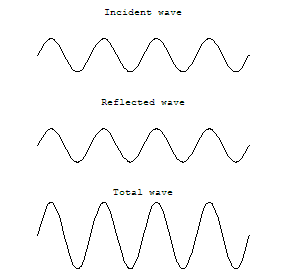
\includegraphics[width=\textwidth]{sin-1}
                \caption{}
                \label{fig:standing_wave:frame_1}
        \end{subfigure}%
        ~ %add desired spacing between images, e. g. ~, \quad, \qquad, \hfill etc.
          %(or a blank line to force the subfigure onto a new line)
        \begin{subfigure}[b]{0.23\textwidth}
                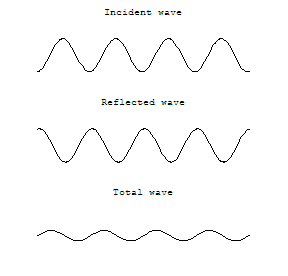
\includegraphics[width=\textwidth]{sin-2}
                \caption{}
                \label{fig:standing_wave:frame_2}
        \end{subfigure}
        ~ %add desired spacing between images, e. g. ~, \quad, \qquad, \hfill etc.
          %(or a blank line to force the subfigure onto a new line)
        \begin{subfigure}[b]{0.23\textwidth}
                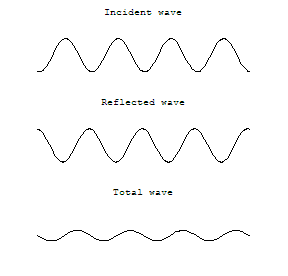
\includegraphics[width=\textwidth]{sin-3}
                \caption{}
                \label{fig:standing_wave:frame_3}
        \end{subfigure}
        ~ %add desired spacing between images, e. g. ~, \quad, \qquad, \hfill etc.
          %(or a blank line to force the subfigure onto a new line)
        \begin{subfigure}[b]{0.23\textwidth}
                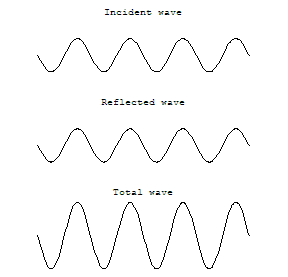
\includegraphics[width=\textwidth]{sin-4}
                \caption{}
                \label{fig:standing_wave:frame_4}
        \end{subfigure}
        \caption{Ukázka principu stojaté vlny. Pvní vlna směřuje zleva do prava, po odrazu změní fázi a směřuje zprav do leva (zobrazena jako druhá vlny). Výsledná vlna je vykreslena jako třetí.}\label{fig:standing_wave}
\end{figure}

Čtenář si může povšimnout, že u výsledné vlny jsou body, které neosciluji, stojí na místě, tyto body se nazívají uzly. Místu
kde vlná kmitá nejvíce, mezi minimem a maximem, říkamé kmity.
U viditelného světla je tato oscilace tak rychlá, že lidské oko
detekuje pouze průmernou světlost vlny. Světlo není tam kde jsou uzly a místo se jeví jako tmavé, zatímco kmity se jeví jako světlé.
Na obrázku \ref{fig:intensityvsamplitude} je znázorněno jak by takovéto chování mohlo vypadat.

\begin{figure}[!htb]
   \centering
 	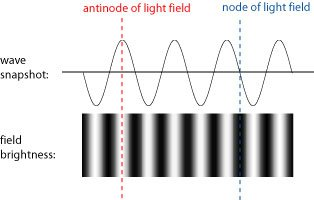
\includegraphics{intensityvsamplitude}
   \caption{Intenzita světla pro kmity a uzly. Kmity jsou světlá místa. Uzly jsou tmavá místa.}
   \label{fig:intensityvsamplitude}
\end{figure}

Jistě stojí za zmínku, že vzdálenost mezi uzly a kmity je 
práve polovina vlnové délky. Pozice uzlů a kmitů je určena tím
zda-li vlna po odrazu mení či nemění znaménko (fázi). Změna fáze je 
znázorněna na obrázku \ref{fig:eh_reflection}

\begin{figure}[!htb]
   \centering
 	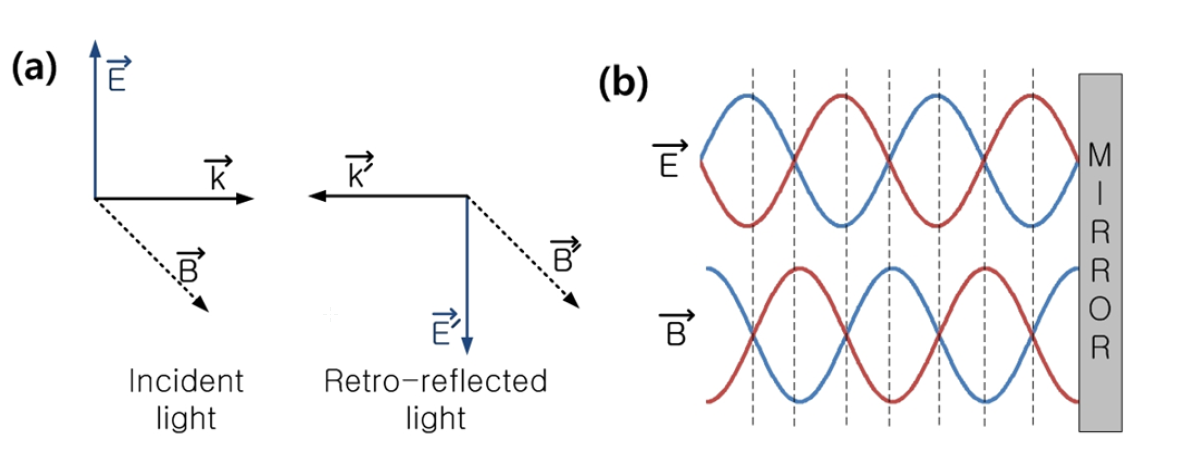
\includegraphics[width=\textwidth]{eh_reflection}
   \caption{Změna fáze světla pri odrazu.}
   \label{fig:eh_reflection}
\end{figure}

Paprsek světla je tvořem dvěmi částmi. Jedná se o elekrickou složku
$E$ a magnetickou složku $H$. Obě tyto složky oscilují se stejnou
vlnovou dělkou, frekvencí a jsou ve fázi (viz obrázek \ref{fig:ehpropagation}), mohou také indukovat jak elekrické tak magnetické sily podle Lorentzova zákova sily
\begin{equation}
F = e(E+\frac{v}{c}\times B)
\end{equation}

\begin{figure}[!htb]
   \centering
 	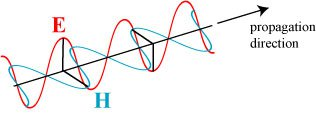
\includegraphics{ehpropagation}
   \caption{Propagace elekrické a magnetické části světla.}
   \label{fig:ehpropagation}
\end{figure}

V optice se můžeme setkat s tím, že u světla se znázorňuje pouze jeho
elekrická část, také polarizace světla se určuje podle směru elekrické složky. Magnetická složka je povětšinou ignorována.

\section{Wienerův pokus}
\todo{nejak to podat}
V roce 1890 nebyla úplně známá strutůra atomu a nebyl zcela zřejmé
chápaní jak svělo interaguje s hmotou. Hlavní otázkou bylo, zda-li
v chemických procesech při výrobě fotografii je spíše zapojeno 
$E$ nebo $H$.

A major question remained unanswered: how the vibration phase changes when light is incident perpendicularly. Inspired by Hertz’s work, Wiener hoped to find an answer and, if possible, to demonstrate standing light waves. He did, in fact, succeed in making visible nodes and antinodes separated by intervals of about 2 . 10-5 centimeters in front of a plane silver plate on which monochromatic light shone perpendicularly. He achieved this with a suitably mounted photosensitive plate, like those used in photography, the thickness of which was about 1/30; the wavelengths. Wiener demonstrated conclusively that it was the nodes of the resulting light vibrations. and not antinodes. that lay in the mirror surface. Accordingly, the reflection of light must take place with phase inversion: this was the answer to his question. In addition the experiment revealed that only the electric portion of the electromagnetic light waves blackens the silver chloride in the photosensitive layer. Wiener’s amazing success was acknowledged as a masterpiece of experimentation.

Wiener developed the following experiment, depicted below, to specify the role of the electric field in optics \ref{fig:energy_fig_wiener}

\begin{figure}[!htb]
   \centering
 	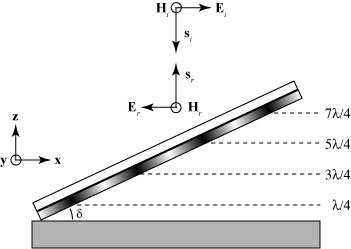
\includegraphics{energy_fig_wiener}
   \caption{Nákres Wienerova pokusu.}
   \label{fig:energy_fig_wiener}
\end{figure}

Monochromatická polorizovaná vlna směřuje kolmo na odrazovou plochu. V tomto
projektu předpokládáme dokonalé zrcadlo (z důvodu zachovaní jednoduchosti). Vlna mířící na zrcadlo společne s odraženo vlnou
vytvoří stojatou vlnu. Wiener použil tenky film (fimly by měl být výrazně tenčí než vlnová délka světla). 
Na filmu se mohly objevit dva vzory. Pokud se podívate na obrázek \ref{fig:energy_fig_wiener}, na výsledném filmu mohly být světlé a tmavé vertikální čáry, v případě, že film ovlivňuje elekrická část světla (to proto, že v prostoru z pohledu zhora, stejně jako na obrázku, se střídají světlé a tmavé proužky ve směru osy $z$). Pokud by se na filmu objevily 
horizontální světlé a tmavé proužky, znamenalo by to, že film byl ovlivněn magnetickou částí světla (to proto, že v prostoru z pohledu zhora, stejně jako na obrázku, se střídají světlé a tmavé proužky ve směru osy $y$). Pokud by byl fiml pod uhlem 0 (rovnoběžne se srcadlem) nejenom, že by výsledek nešel vidět pouhym okem, ale také by byl film buď světlý nebo tmavý. Zde Wiener použil chytrý trik, pri kterém film natočil o malý úhel. To způsobilo, že film nyní \emph{prořezává} světlé a tmavé vsrtvy, čimž dochází k pojekci 
na film.

Na povrchu zrcadla, musí být elekrická část světla rovna nule, zatímco magnetická část zde nabýva svého maxima. Jednoduše se dá 
vypočíst, že maxima elekrické složky v ose $z$ budou
\begin{equation}
z = m\lambda / 4, \quad m=1,2,3,\ldots
\end{equation}
zatímco maxima magnetické složky se nachází
\begin{equation}
z = m\lambda / 4, \quad m=2,4,6,\ldots
\end{equation}

Kde $\lambda$ vyjadřuje vlnovou délku světla. Z rovnich vyplývá, že
maxima elekrické a magnetické složky se objevují v jiných bodech prostoru. Pozorováním filmu, může být pomocí světlých a tmavých proužků vyvozeno, zda-li má vliv elekrická nebo magnetická složka světla v chemických procesech při tvorbě fotografie.

Wiener tímto demonstroval, kontextu s elekromagnetickou teorii, že elekrická část světla je hlavní (důležitější) části světla.

Wiener měl před sebou ješte jednu překážku to film. Ten nejenom, že musel bý průhledný, aby mohlo světlo procházet zkrz, ale také dostatečné tenký (významně tenčí než vlnová délka světla).
Wiener ve svém experimentu použil film, který byl asi 30x tenčí než 
vlnová delká světla které použival (sodiová oblouková lampa, přibližně s 600 $nm$). Film měl tedy přobližne okolo 20 $nm$.

\section{Popis aplikace}
\lipsum[40]

\section{Závěr}
\lipsum[50]
\lipsum[51]
\lipsum[52]

\textcolor{white}{
	\citep{klingmann_thesis}
	\cite{he}
	\cite{zhang}
	\cite{ann}
}


\bibliographystyle{plain}
\bibliography{references}
\end{document}
